\subsection{Functions} \label{subsec:functions}

\begin{figure*}[!ht]
    \centering
    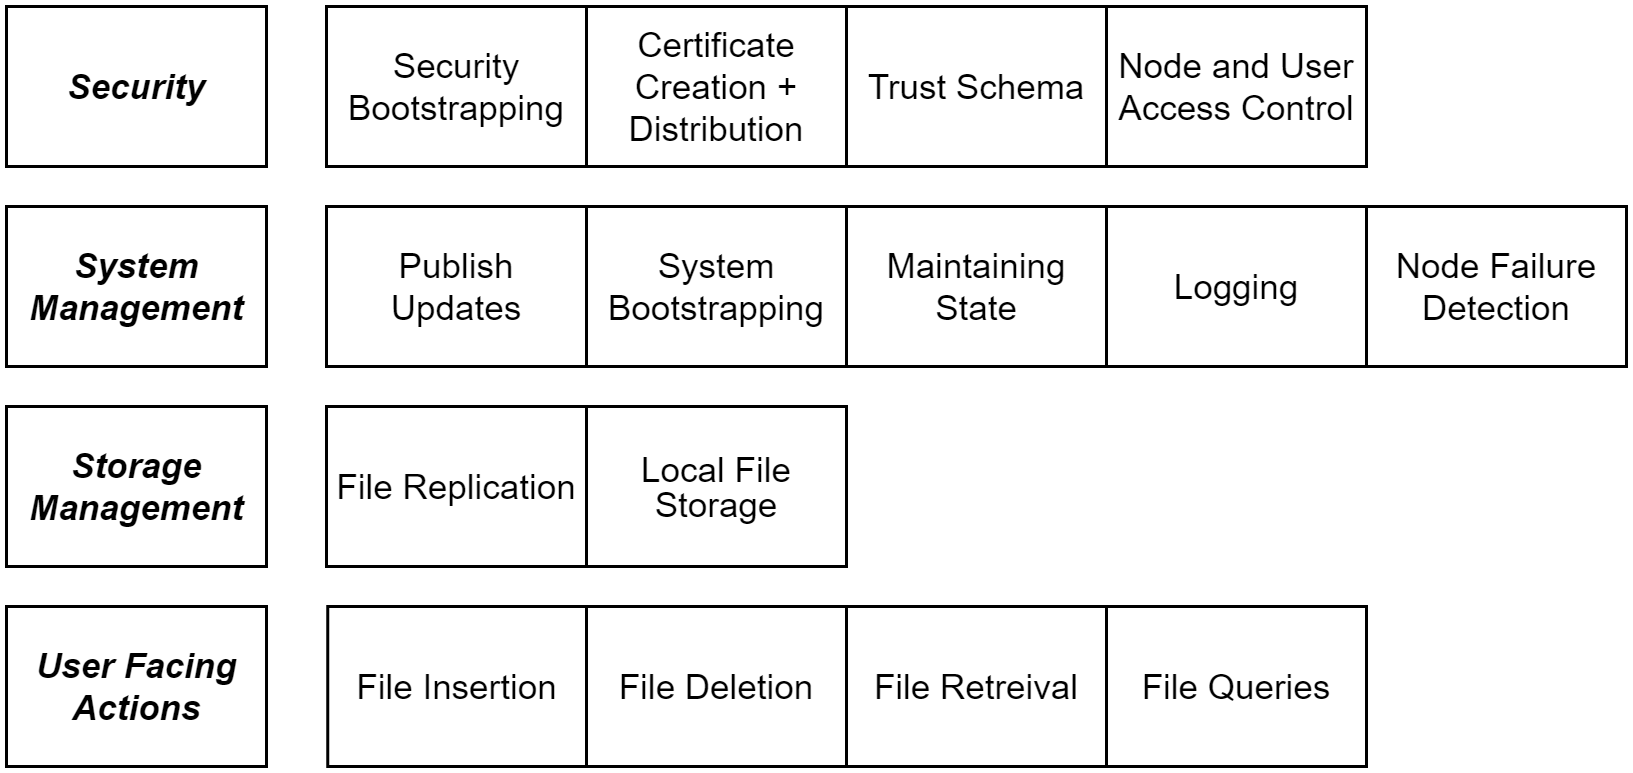
\includegraphics[width=2\columnwidth]{visuals/node-functions.png}
    \caption{Necessary Functions of a Hydra Node}
    \label{fig:node-functions}
\end{figure*}
%\todo[inline]{This needs to be updated. Remove the lines, and make sure the boxes are correct. - Justin}

As Figure~\ref{fig:overview} outlines, a Hydra federation has four types of functions:

\begin{itemize}
    \item Bootstrapping
    \item System Management
    \item Storage Management
    \item User Facing Functions
\end{itemize}

Figure~\ref{fig:node-functions} outlines each of these categories.
%and what exact functions go into them. An explanation of these categories and further references follow.

\subsubsection{Bootstrapping} can be divided into security bootstrapping and system bootstrapping. Security bootstrapping focuses on getting proper key and certificate information that the node can present to the federation before it is allowed to join. We discuss bootstrapping in Section   \ref{sec:node-operations}. System bootstrapping focuses on the functionality needed for a new node to join the federation and sync the node's state to the system's state. 

\subsubsection{System Management} modules provide the necessary systems level functionality for Hydra. These include maintaining states in the network, publishing and applying updates to the system state, 
% user access control (NOTE: this should go to security), 
logging, node failure detection, and failure recovery. These functions are at the core of how Hydra operates. Management of system is discussed further in Section \ref{sec:node-operations}.

\subsubsection{Storage Management} functions oversee file replication and local file storage. The file replication module replicates files across Hydra nodes and maintains the degree of replication (currently 3). This ensures data loss does not occur even when individual nodes fail. The local file storage module handles the storage functions of a node. These include interacting with the underlying database or filesystem, and freeing up storage by deleting unused files.
%Both functions are necessary for maintaining copies of uploaded files throughout the system, ensuring data is not lost. 
Further discussion on file replication can be found in Section \ref{sec:data-operations} and local storage can be found Section \ref{subsec:modules}.

\subsubsection{User Facing functions} provide user interfaces for various user and application interactions. These functions include file insertion, deletion, retrieval, and system status checks. Hydra exposes name-based APIs for these functions that can be directly used by the users or integrated into separate applications. More details on user facing functions can be found in Section \ref{sec:data-operations}.